\chapter{YouTube}
\label{ch:youtube}

\begin{gram}[Introduction]
\label{grm:youtube:introduction}
    YouTube is another option for distributing course content.
    %
    YouTube has recently been enabled with you CMU Andrew GSuite account.
    %
    Faculty, staff, and students: Log into \href{https://www.youtuube.com/}{https://www.youtube.com/} using your Andrew ID and password.

    \begin{note}[Help resources]
        Browse \href{https://www.youtube.com/user/youtubehelp?sub_confirmation=1}{YouTube's video library} for feature overviews and step-by-step tutorials.
        %
        If you get stuck, please contact the Video Services Team at \href{mailto:coursecast@cs.cmu.edu}{coursecast@cs.cmu.edu} for help.
    \end{note}

\end{gram}


\section{Getting Started}
\label{sec:youtube:getting_started}

\begin{gram}[Uploading Content to YouTube]
    Videos must be saved locally and then uploaded manually to YouTube.
    %
    Click ``Create'' to upload a new video.
    %
    The upload process will prompt you to add a video title and description, customize visibility sttings, and adjust other settings.

    {
        \centering
        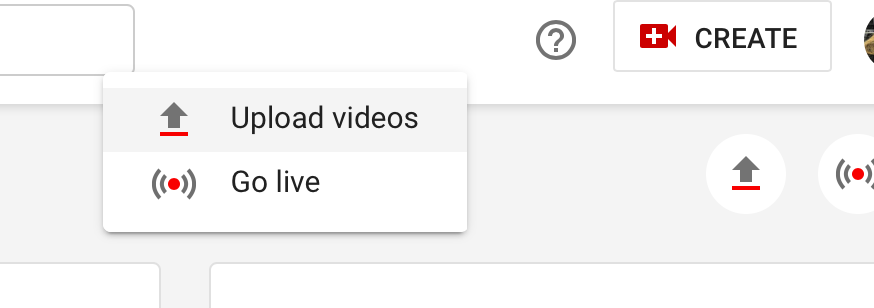
\includegraphics[scale=0.4]{youtube/media/08-youtube-upload.png}
    }
\end{gram}

View the video below for a step-by-step guide:

\video{https://www.youtube.com/watch?v=klVWGHtRTuE}{Upload to YouTube}

\begin{note}[Video Editing in Panopto + YouTube]
    You may have \href{sec:panopto:editing_videos}{edited a video} in Panopto.
    %
    Panopto videos can be downloaded locally and uploaded to YouTube.
    %
    \href{https://www.panopto.com/blog/how-to-upload-a-panopto-video-to-youtube/}{This guide} explains how.
    %
    If your Panopto video has been edited using Panopto's internal editor, then these edits will be reflected in your downloaded video.
\end{note}

\begin{gram}[YouTube Studio]
    Navigate to YouTube Studio.
    %
    Here, you can customize your channel dashboard, create playlists, and adjust individual video settings (descriptions, visibility, thumnbnails, etc.).
    %
    Click on your user icon in the top right corner and select YouTube Studio from the drop-down menu.
    %
    You can also navigate to \href{https://studio.youtube.com/}{https://studio.youtube.com/}.

    {
        \centering
        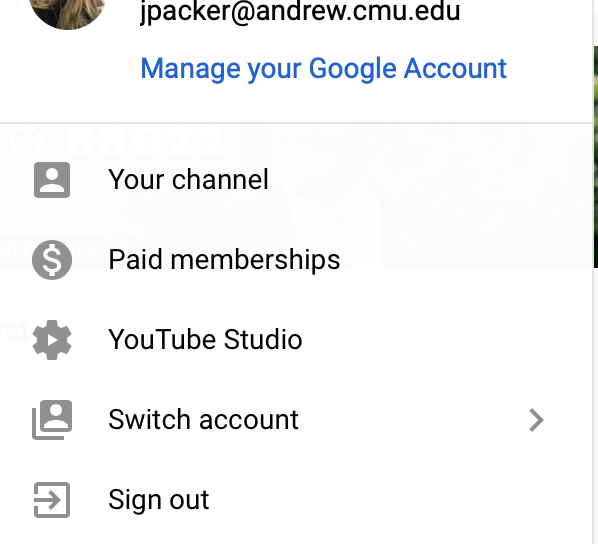
\includegraphics[scale=0.4]{youtube/media/09-youtube-studio.png}
    }
\end{gram}


\section{Visibility Settings}
\label{sec:youtube:visibility settings}

YouTube offers the following visibility settings:

\begin{itemize}
        \item \textbf{Private.} ``Only you and people you choose can watch your video.''
        \item \textbf{Unlisted.} ``Anyone with the video link can watch your video.''
        \item \textbf{Public.} ``Everyone an watch your video.''
    \end{itemize}

This video explains YouTube's visibility settings in detail:

\video{https://www.youtube.com/watch?v=_j3pGmiKvxU}{How to change video privacy settings on YouTube}

\begin{gram}[Where to adjust visibility settings]
    You will be prompted to select ``Private'', ``Unlisted'', or ``Public'' every time you upload a new video.
    %
    The video below explains how to customize your default upload visibility settings.
    %
    To re-adjust privacy settings for a video that has already been uploaded: Navigate to YouTube Studio > Videos > click on your video's thumbnail to adjust Video Details > see the visibility drop-down menu on the right-hand side of the Video Details dashboard.

    \video{https://www.youtube.com/watch?v=kuplp_Gd7xg}{Customize your upload preferences on YouTube}
\end{gram}

\begin{gram}[Student and Organizational Access]
    It is possible to restrict video access to either students/course particpants or CMU affiliates.
    %
    First, upload a video and set its visibility to ``Private.''
    %
    Next, go to YouTube Studio > Videos > click on your Video's thumbnail > in Video Details, click Options (3 vertical dots) > select Share Prviately.

    {
        \centering
        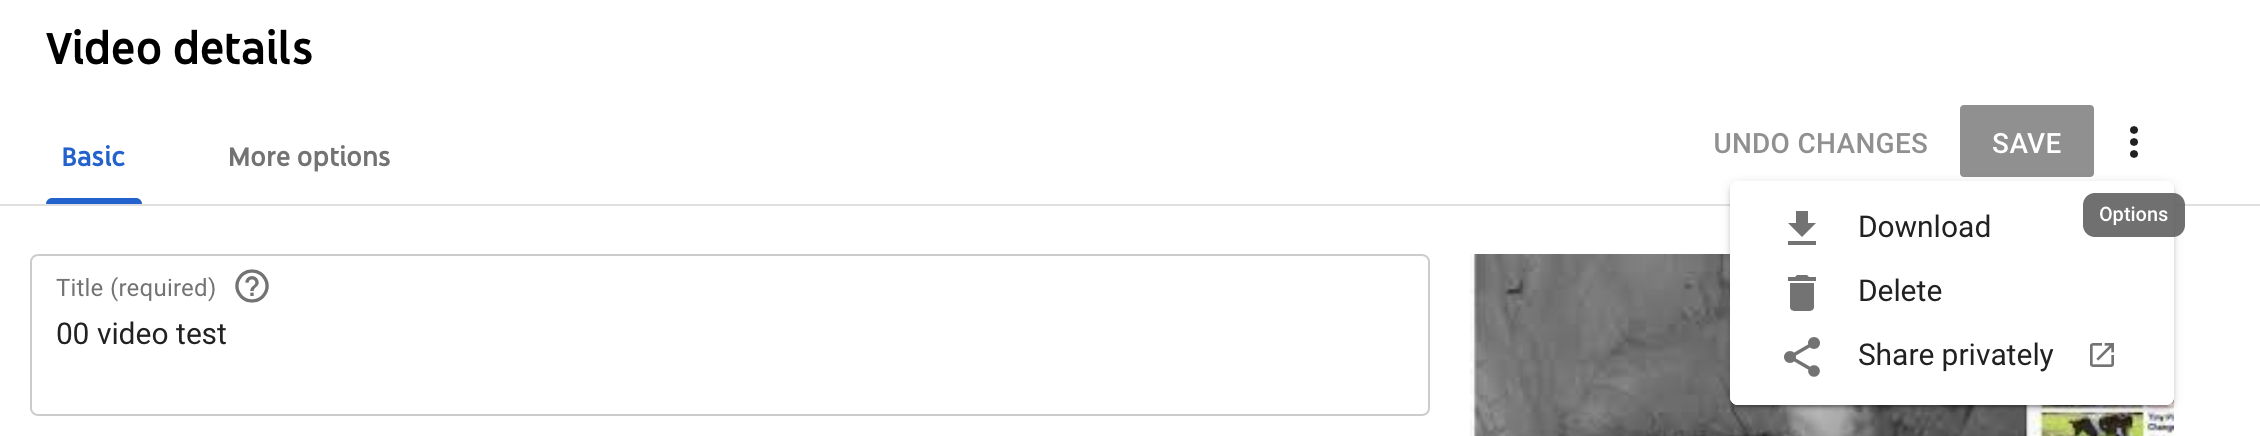
\includegraphics[scale=0.4]{youtube/media/10-youtube-private-access-1.png}
    }

    The following screen will appear.
    %
    If you want to restrict your video to course participants, then you will need to enter participants' email addresses manually.
    %
    To implement organizational access, check the box to restrict to ``andrew.cmu.edu'' viewers.

    {
        \centering
        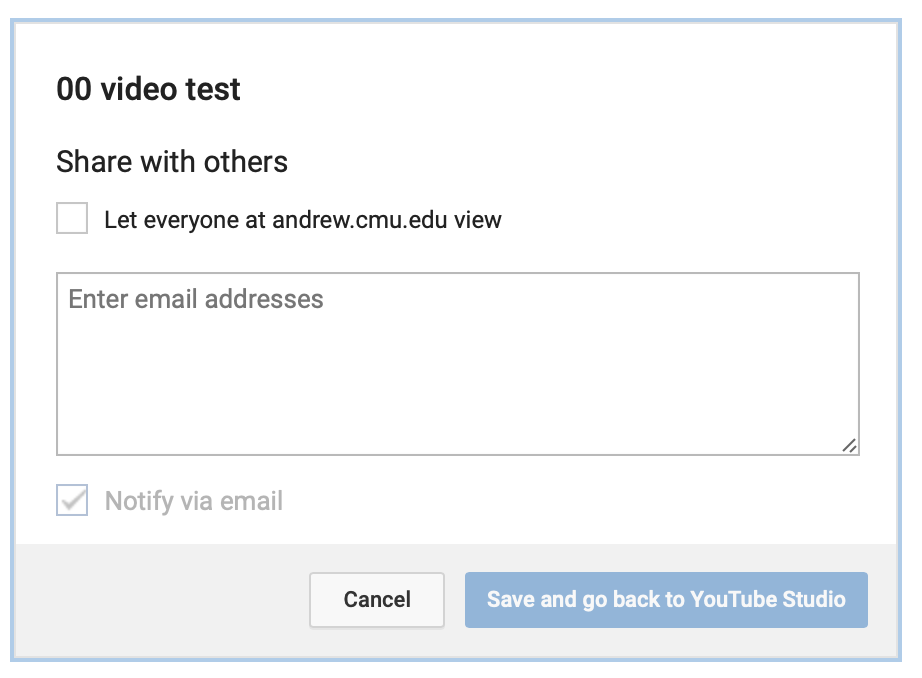
\includegraphics[scale=0.4]{youtube/media/11-youtube-private-access-2.png}
    }
\end{gram}